\title{คาบเรียนที่ 9: รูปแบบไม่กำหนด และ ปริพันธ์ \\ (Indeterminate form and integral)}
\frame{\titlepage}

\begin{frame}{สารบัญ}
\tableofcontents
\end{frame}

%%%%%%%%%%%%%%
\section{รูปแบบไม่กำหนด}
\frame{\sectionpage}
%%%%%%%%%%%%%%

\begin{frame}
\frametitle{การหาลิมิตเมื่อแทนค่าไม่ได้}
พิจารณาลิมิต 
\[ \lim_{x \to 0} \frac{1}{x} \]
ซึ่งเราทราบทันทีว่าลู่ออก เพราะแทนค่า $x=0$ แล้วจะหาค่าไม่ได้ แต่
\[ \lim_{x \to 0} \frac{\sin x}{x} \]
เราบอกไม่ได้ในทันทีว่ามีลิมิตหรือไม่ เพราะเมื่อแทนค่า $x=0$ แล้วจะได้ $\frac{0}{0}$ ซึ่งเป็นไปได้ว่าเราสามารถกำจัดเศษและส่วนออกจากกัน แล้วทำให้ลิมิตหาค่าได้
\end{frame}

\begin{frame}
\frametitle{รูปแบบไม่กำหนด}
ในที่นี้ เราจะมาจำแนกว่าลิมิตประเภทใดที่อยู่ในรูปที่\red{อาจจะ}หาค่าได้
\begin{defn}{}{}
รูปแบบไม่กำหนด (Indeterminate Form) มีทั้งหมด 7 รูปแบบด้วยกัน ได้แก่
\[ \frac{0}{0}, \quad \frac{\infty}{ \infty}, \quad \infty \times 0, \quad \infty - \infty, \quad 1^{\infty}, \quad 0^0, \quad \infty^0 \]
\end{defn}
\begin{remark}{ข้อควรระวัง}
เราใช้การแทนค่าเพื่อตรวจสอบรูปแบบเท่านั้น แต่จะไม่เขียนรูปแบบเหล่านี้ในสมการ จะติดในรูปของลิมิตเสมอ จนกว่าจะสรุปได้ว่าลู่เข้าหรือลู่ออก
\end{remark}
\end{frame}


\begin{frame}[t]
\begin{ex}
จงหาว่าลิมิตใดต่อไปนี้อยู่ในรูปแบบไม่กำหนดหรือไม่
\begin{tasks}(3)
\task $\limx{1} \frac{x^4-1}{x-1}$
\task $\limx{1} \frac{x^4+1}{x-1}$
\task $\limx{0} \frac{2^{1/x}}{3^{1/x}}$
\end{tasks}
\end{ex}
\end{frame}

\begin{frame}
\begin{sol}
\begin{tasks}(1)
\task เมื่อแทนค่า $x=1$ จะได้ $\frac{1^4-1}{1-1} = \frac{0}{0}$ ซึ่งเป็นรูปแบบไม่กำหนด
\task เมื่อแทนค่า $x=1$ จะได้ $\frac{1^4+1}{1-1} = \frac{2}{0}$ ซึ่ง\red{ไม่}เป็นรูปแบบไม่กำหนด นั่นคือเราสรุปได้ทันทีว่าลิมิตลู่ออก
\task เมื่อแทนค่า $x=0$ จะได้ $\frac{2^{1/0}}{3^{1/0}} = \frac{2^{\infty}}{3^{\infty}} = \frac{\infty}{\infty}$ ซึ่งเป็นรูปแบบไม่กำหนด
\end{tasks}
\end{sol}
\end{frame}


\begin{frame}[t]
\begin{ex}
จงหาว่าลิมิตใดต่อไปนี้อยู่ในรูปแบบไม่กำหนดหรือไม่
\begin{tasks}[style=enumerate](2)
\task $\limx{\infty} \sqrt{x+1} - \sqrt{x}$
\task $\limx{\infty} \left(\frac{1}{x}\right)^x$
\end{tasks}
\end{ex}
\end{frame}

\begin{frame}
\begin{sol}
\begin{tasks}[style=enumerate](1)
\task เมื่อแทนค่า $x= \infty$ จะได้ $\sqrt{\infty + 1} - \sqrt{\infty} = \infty - \infty$ ซึ่งเป็นรูปแบบไม่กำหนด
\task เมื่อแทนค่า $x=\infty$ จะได้ $\left(\frac{1}{\infty}\right)^{\infty} = 0^{\infty}$ ซึ่งเป็นรูปแบบไม่กำหนด
\end{tasks}
\end{sol}
\end{frame}


\begin{frame}
แม้ว่าลิมิตจะอยู่ในรูปแบบไม่กำหนด เราก็ยังไม่ทราบว่าหาลิมิตได้หรือไม่ เช่น
\begin{tasks}[style=enumerate](1)
\task $\limx{\infty} \frac{x+1}{x^2+1} \begin{slide}= 0 \end{slide}$
\task $\limx{\infty} \frac{x^2+1}{x+1} \begin{slide}=+ \infty \end{slide}$
\task $\limx{\infty} \frac{x^2+1}{x^2-1} \begin{slide}=1\end{slide}$
\end{tasks}
สังเกตว่า มีค่าที่เป็นไปได้หลายแบบ แต่การที่จะต้องไล่ทดลองวิธีการต่าง ๆ เช่น แยกตัวประกอบ ดึงตัวร่วม คูณด้วยสังยุค ใช้เอกลักษณ์ตรีโกณมิติ ฯลฯ จะต้องใช้เวลา เราจึงต้องเสาะหาเครื่องมือใหม่มาช่วยในการคำนวณ
\end{frame}

%%%%%%%%%%%%%%
\section{กฎของโลปิตาล}
\frame{\sectionpage}
%%%%%%%%%%%%%%

\begin{frame}
%\frametitle{กฎของโลปิตาล}
\begin{thm}{}{}
ให้ $f,g$ เป็นฟังก์ชันที่หาอนุพันธ์ได้ที่ $c$
\begin{tasks}[style=enumerate](1)
\task ถ้า $\limx{c} f(x) = 0 = \limx{c} g(x)$ \pa แล้ว
\begin{equation} \label{eq:lhopital1}
 \limx{c} \frac{f(x)}{g(x)} = \limx{c} \frac{f\,'(x)}{g\,'(x)}
 \end{equation}
\task ถ้า $\limx{c} f(x) = \pm\infty$ และ $\limx{c} g(x) = \pm \infty$ \pa แล้ว
\begin{equation} \label{eq:lhopital2}
\limx{c} \frac{f(x)}{g(x)} = \limx{c} \frac{f\,'(x)}{g\,'(x)}
\end{equation}
\end{tasks}
\end{thm}
\end{frame}


\begin{frame}[t]
\begin{ex}
จงหา $\limx{0} \frac{x^2+3x}{x}$ โดยกฎของโลปิตาล
\end{ex}\pa 
\begin{sol}
สังเกตว่าถ้าให้ $f(x) = x^2+3x$ และ $g(x) = x$ แล้ว $\limx{0} f(x) = 0 = \limx{0} g(x)$ \pa ฉะนั้นเราจึงไม่สามารถแทนค่า $x=0$ ได้ทันที \pa

จากกฎของโลปิตาล จะได้ว่า
\begin{eqnarray*}
\limx{0} \frac{x^2+3x}{x} \pa &=& \limx{0} \frac{\dx (x^2+3x)}{\dx (x)} \pa \\
&=& \limx{0} \frac{2x+3}{1} \pa \\
&=& (2)(0) + 3 = 3
\end{eqnarray*}
\end{sol}
\end{frame}


\begin{frame}[t]
\begin{ex}
จงหา $\limx{1} \frac{x^3-x}{x^2-3x+2}$ โดยกฎของโลปิตาล
\end{ex}\pa 
\begin{sol}
สังเกตว่าถ้าให้ $f(x) = x^3-x$ และ $g(x) = x^2-3x+2$ แล้ว $\limx{1} f(x) = 0 = \limx{1} g(x)$ \pa ฉะนั้นเราจึงไม่สามารถแทนค่า $x=1$ ได้ทันที \pa

จากกฎของโลปิตาล จะได้ว่า
\begin{eqnarray*}
\limx{1} \frac{x^3-x}{x^2-3x+2} \pa = \limx{1} \frac{\dx (x^3-x)}{\dx (x^2-3x+2)} \pa &=& \limx{1} \frac{3x^2-1}{2x-3} \pa \\
&=& \frac{3(1)^2 - 1}{2(1) - 3} \pa \\
&=& \frac{2}{-1} = -2
\end{eqnarray*}
\end{sol}
\end{frame}


\begin{frame}[t]
\begin{ex}
จงหา $\limx{\infty} \frac{5x^2+12}{-x^2+56}$ โดยกฎของโลปิตาล
\end{ex}\pa 
\begin{sol}
สังเกตว่าถ้าให้ $f(x) = 5x^2+12$ และ $g(x) = -x^2+56$ \pa แล้ว $\limx{\infty} f(x) = \infty$ และ $ \limx{\infty} g(x) = -\infty$ \pa เราจึงไม่สามารถหาลิมิตของตัวเศษและส่วนแยกกันได้

จากกฎของโลปิตาล จะได้ว่า
\begin{eqnarray*}
\limx{\infty} \frac{5x^2+12}{-x^2+56} \pa &=& \limx{\infty} \frac{\dx(5x^2+12)}{\dx (-x^2+56)} \pa \\
&=& \limx{\infty} \frac{10x}{-2x} \pa \\
&=& \limx{\infty} -5 \pa \\
&=& -5
\end{eqnarray*}
\end{sol}
\end{frame}


\begin{frame}[t]
\begin{ex}
จงหา $\limx{0} \frac{e^x-1-x}{x^2}$ โดยกฎของโลปิตาล
\end{ex}\pa 
\begin{sol}
สังเกตว่าถ้าให้ $f(x) = e^x-1-x$ และ $g(x) = x^2$ \pa แล้ว $\limx{0} f(x) = 0 = \limx{0} g(x)$ ฉะนั้นเราจึงไม่สามารถแทนค่า $x=0$ ได้ทันที \pa

จากกฎของโลปิตาล จะได้ว่า \pa
\[ \limx{0} \frac{e^x-1-x}{x^2} = \limx{0} \frac{e^x-1}{2x} \] \pa
แต่ว่า! เรายังหาค่าของลิมิตไม่ได้อยู่ดี เพราะว่า $\frac{e^0 - 1}{2\cdot 0} = \frac{0}{0}$ \pa ถึงกระนั้น เราสามารถใช้กฎของโลปิตาลกับลิมิต $\limx{0} \frac{e^x-1}{2x}$ ได้อีกรอบ
\end{sol}
\end{frame}

\begin{frame}[t]
\begin{sol} (ต่อ)
ถ้าให้ $f_2(x) = e^x-1$ และ $g_2(x) = 2x$ \pa แล้ว $\limx{0} f_2(x) = 0 = \limx{0} g_2(x)$
\begin{eqnarray*}
\limx{0} \frac{e^x-1}{2x} \pa &=& \limx{0} \frac{e^x}{2}\pa \\
&=& \frac{e^0}{2} = \frac{1}{2} \pa
\end{eqnarray*}
ฉะนั้น 
\[ \limx{0} \frac{e^x-1-x}{x^2} \pa = \limx{0} \frac{e^x-1}{2x} \pa = \frac{1}{2} \]
\end{sol}
\end{frame}

%%%%%%%%%%%%%%
\section[$0 \times \infty$]{เทคนิคการจัดรูป เมื่อลิมิตอยู่ในรูปแบบ $0 \times \infty$}
\frame{\sectionpage}
%%%%%%%%%%%%%%

\begin{frame}
แม้ว่ากฎของโลปิตาลจะอยู่ในรูปแบบของผลหาร แต่เราสามารถจัดรูปลิมิตอื่นให้กลายเป็นรูปแบบของผลหารได้ ดังนี้
\begin{thm}{}{}
กำหนดฟังก์ชัน $u(x)$ และ $v(x)$ ที่ $\limx{c} u(x) = 0$ และ $\limx{c} v(x) = \infty$ จะได้ว่า
\begin{equation}
\limx{c} u(x) v(x) = \limx{c} \frac{u(x)}{\left( \frac{1}{v(x)} \right)}
\end{equation} \pa
ซึ่งเป็นรูปแบบไม่กำหนดในรูป $\frac{0}{0}$ ที่ใช้กฎโลปิตาลในการหาค่าของลิมิตได้
\end{thm}
\end{frame}


\begin{frame}[t]
\begin{ex}
จงหา $\limx{0} x \ln x$ โดยกฎของโลปิตาล
\end{ex}\pa 
\begin{sol}
สังเกตว่าเมื่อแทนค่า $x=0$ แล้วจะอยู่ในรูป $0 \cdot (-\infty)$ ฉะนั้นเราจึงจัดรูปก่อนเป็น
\[ x \ln x = \frac{\ln x}{\left( \frac{1}{x} \right)}\] \pa
ในเมื่อเราได้รูปแบบ $\frac{\infty}{\infty}$ มาแล้ว จึงสามารถใช้กฎของโลปิตาลได้
\begin{eqnarray*}
\limx{0} \frac{\ln x}{\left( \frac{1}{x} \right)} \pa = \limx{0} \frac{\dx (\ln x)}{\dx (1/x)} &=& \limx{0} \frac{ \frac{1}{x}}{ -\frac{1}{x^2}} \pa \\
&=& \limx{0} -x\pa \\
&=& 0
\end{eqnarray*}
\end{sol}
\end{frame}




\begin{frame}[t]
\begin{ex}
จงหา $\limx{\infty} x e^{-x} $ โดยกฎของโลปิตาล
\end{ex}\pa 
\begin{sol}
สังเกตว่าเมื่อแทนค่า $x=0$ แล้วจะอยู่ในรูป $\infty \cdot 0$ ฉะนั้นเราจึงจัดรูปก่อนเป็น
\[x e^{-x} = \frac{x}{e^x}\] \pa
ซึ่งเป็นรูปเศษส่วนที่อยู่ในรูปแบบ $\frac{\infty}{\infty}$ ฉะนั้นเราใช้กฎของโลปิตาลได้ดังนี้
\begin{eqnarray*}
\limx{\infty} x e^{-x} \pa = \limx{\infty} \frac{x}{e^x} &=& \limx{\infty} \frac{\dx x}{\dx e^x} \\
&=& \limx{\infty} \frac{1}{e^x}  \\
&=& 0
\end{eqnarray*}
\end{sol}
\end{frame}

%%%%%%%%%%%%%%
\section[$\infty - \infty$]{เทคนิคการจัดรูป เมื่อลิมิตอยู่ในรูปแบบ $\infty - \infty$}
\frame{\sectionpage}
%%%%%%%%%%%%%%

\begin{frame}
รูปแบบไม่กำหนด 
\[ \infty - \infty\]
แม้อาจจะดูเหมือนได้ 0 แต่ต้องระวังว่าที่จริงแล้ว $\infty$ ไม่ใช่จำนวน จึงเอามาลบกันไม่ได้ ลิมิตต่อไปนี้อยู่ในรูปแบบ $\infty - \infty$ เหมือนกันหมด แต่มีค่าต่างกัน เช่น
\begin{eq*}
\limx{\infty} 2x - x &=& \begin{slide}+\infty \end{slide}\\
\limx{\infty} x - x &=&\begin{slide} 0\end{slide} \\
\limx{\infty} (x+1) - x &=& \begin{slide}1\end{slide} \\
\limx{0} \frac{1}{x} - \frac{1+x}{x} &=& \begin{slide}-1\end{slide}
\end{eq*}
\end{frame}

\begin{frame}
\begin{remark}{}
กำหนดฟังก์ชัน $u(x)$ และ $v(x)$ ที่ $\limx{c} u(x) = \limx{c} v(x) = \infty$ ในการหาลิมิต
\[\limx{c} u(x) - v(x)\]
ให้จัดรูปด้วยวิธีใดวิธีหนึ่งดังต่อไปนี้
\begin{tasks}(1)
\task บวกลบเศษส่วนรวมกัน จนได้เป็นเศษส่วนเดียวในรูปแบบไม่กำหนด $\frac{0}{0}$ หรือ $\frac{\infty}{\infty}$
\task คูณ $u(x) - v(x)$ ด้วยสังยุค $u(x) + v(x)$ ทั้งตัวเศษและตัวส่วน
\task อื่น ๆ
\end{tasks}
และใช้กฎโลปิตาลในการหาค่าของลิมิตต่อไป
\end{remark}
\end{frame}



\begin{frame}[t]
\begin{ex}
จงหา $\limx{\infty} \ln (x+1) - \ln x $ โดยกฎของโลปิตาล
\end{ex}\pa 
\begin{sol}
สังเกตว่าเมื่อแทนค่า $x=\infty$ แล้วจะอยู่ในรูป $\infty - \infty$ แต่ว่าในที่นี้เราไม่จำเป็นต้องใช้กฎของโลปิตาล สามารถใช้สมบัติของฟังก์ชันลอการิทึมได้ดังนี้
\begin{eq*}
\limx{\infty} \ln (x+1) - \ln x &=& \limx{\infty} \ln \left( \frac{x+1}{x} \right) \\
&=& \limx{\infty} \ln \left(1 + \frac{1}{x}\right) \\
&=& \ln (1 + 0) \\
&=& 0
\end{eq*}
\end{sol}
\end{frame}


\begin{frame}[t]
\begin{ex}
จงหา $\limx{\infty} \sqrt{x^2+3x} - x $ โดยกฎของโลปิตาล
\end{ex}\pa 
\begin{sol}
สังเกตว่าเมื่อแทนค่า $x=\infty$ แล้วจะอยู่ในรูป $\infty - \infty$ ฉะนั้นเราจึงใช้การคูณด้วยสังยุคในการจัดรูป ได้เป็น
\begin{eq*}
\sqrt{x^2+3x} - x &=& \frac{\sqrt{x^2+3x} + x}{\sqrt{x^2+3x} + x} ( \sqrt{x^2+3x} - x ) \\
&=& \frac{(x^2+3x)-x^2}{\sqrt{x^2+3x} + x} = \frac{3x}{\sqrt{x^2+3x} + x} 
\end{eq*}
ซึ่งอยู่ในรูป $\frac{\infty}{\infty}$ ฉะนั้นสามารถใช้กฎของโลปิตาลเพื่อหาลิมิตได้ดังนี้
\begin{eq*}
\limx{\infty} \frac{3x}{\sqrt{x^2+3x} + x} = \limx{\infty} \frac{3}{ \frac{2x+3}{2\sqrt{x^2+3x}} + 1 }= \frac{3}{1+1} = \frac{3}{2}
\end{eq*}
\end{sol}
\end{frame}



\begin{frame}[t]
\begin{ex}
จงหา $\limx{0^-} \frac{1}{x} - \frac{1}{\sin x} $ โดยกฎของโลปิตาล
\end{ex}\pa 
\begin{sol}
สังเกตว่าเมื่อแทนค่า $x=0$ แล้วจะอยู่ในรูป $\frac{1}{0} - \frac{1}{0} = \infty - \infty$ ฉะนั้นเราจึงจัดรูปใหม่เป็น
\[\frac{1}{x} - \frac{1}{\sin x} = \frac{\sin x - x}{x\sin x}\]
ซึ่งกลายเป็นรูป $\frac{0}{0}$
\end{sol}
\end{frame}

\begin{frame}
\begin{sol} (ต่อ)
\begin{eq*}
\limx{0^-} \frac{1}{x} - \frac{1}{\sin x} &=& \limx{0^-} \frac{\sin x - x}{x\sin x} \\
&=& \limx{0^-} \frac{\cos x -1}{x\cos x - \sin x} \mathnote{ใช้กฎโลปิตาล}\\
&=& \limx{0^-} \frac{-\sin x}{- x \sin x + 2 \cos x} \mathnote{ใช้กฎโลปิตาลอีกครั้งหนึ่ง}\\
&=& \frac{0}{0+2}  \mathnote{แทนค่า $x=0$ ในลิมิตได้แล้ว} \\
&=& 0
\end{eq*}
\end{sol}
\end{frame}




%%%%%%%%%%%%%%
\section[ยกกำลัง]{เทคนิคการจัดรูป เมื่อลิมิตอยู่ในรูปแบบ $0^0, 0^{\infty}, 1^{\infty}$}
\frame{\sectionpage}
%%%%%%%%%%%%%%

\begin{frame}[t]
สุดท้าย ถ้าลิมิตอยู่ในรูปแบบฟังก์ชันเลขชี้กำลัง
\[0^0, \quad 0^{\infty}, \quad 1^{\infty}\]
เราสามารถใช้สมบัติของฟังก์ชันลอการิทึม
\begin{slide}
\[ \ln (a^b) = b \ln a \]
เพื่อเปลี่ยนเลขชี้กำลังลงมาเป็นผลคูณของฟังก์ชันแทนได้ ซึ่งจะทำให้เราสามารถใช้เทคนิคก่อนหน้านี้ในการหาลิมิตต่อไป

ข้อควรระวังคือ ลิมิตที่ได้เป็นของฟังก์ชัน $\ln (a^b)$ จึงต้องแทนค่ากลับอีกที นั่นคือ ถ้าเราได้ว่า
\[ \limx{c} \ln ( u(x)^{v(x)} ) = L\]
แล้วจะได้
\[ \limx{c} u(x)^{v(x)} = e^L\]
\end{slide}
\end{frame}

\begin{frame}
\begin{remark}{}{}
กำหนดฟังก์ชัน $u(x)$ และ $v(x)$ ที่ $\limx{c} u(x)^{v(x)}$ เป็นรูปแบบไม่กำหนด แล้ว
\begin{equation}
\limx{c} \ln \left( u(x)^{v(x)}\right) = \limx{c} v(x) \ln u(x) 
\end{equation}
จะอยู่ในรูปแบบของลิมิตไม่กำหนดในรูปผลคูณ ซึ่งใช้กฎโลปิตาลในการหาค่าของลิมิตได้ ถ้าลิมิตลู่เข้าและมีค่าเท่ากับ
\[ \limx{c} v(x) \ln u(x) = L\]
แล้วจะได้ว่า
\[ \limx{c} u(x)^{v(x)} = e^L\]
\end{remark}
\end{frame}




\begin{frame}[t]
\begin{ex}
จงหา $\limx{0} x^x$ โดยกฎของโลปิตาล
\end{ex}\pa 
\begin{sol}
สังเกตว่าเมื่อแทนค่า $x=0$ แล้วจะอยู่ในรูป $0^0$ ฉะนั้นเราจึงหาลิมิตของฟังก์ชันต่อไปนี้แทน
\[ \limx{0} \ln (x^x) = \limx{0} x \ln x \]
ซึ่งเราทราบจากตัวอย่างก่อนหน้านี้แล้วว่า ลิมิตมีค่าเท่ากับ 0 ฉะนั้น
\[ \limx{0} x^x = e^0 = 1\]
\end{sol}
\end{frame}




\begin{frame}[t]
\begin{ex}
จงหา $\limx{\infty} \left( 1 + \frac{1}{x} \right)^x$ โดยกฎของโลปิตาล
\end{ex}\pa 
\begin{sol}
สังเกตว่าเมื่อแทนค่า $x = \infty$ แล้วจะอยู่ในรูป $1^{\infty}$ ฉะนั้นเราจึงหาลิมิตของฟังก์ชันต่อไปนี้แทน \pa
\[ \limx{\infty} \ln \left( 1 + \frac{1}{x} \right)^x = \limx{\infty} x \ln \left( 1 + \frac{1}{x} \right)\] \pa
ในเมื่อเราได้รูปแบบ $\infty \cdot 0$ มาแทน จึงสามารถจัดรูปและใช้กฎของโลปิตาลได้
\begin{eqnarray*}
\limx{\infty} x \ln \left( 1 + \frac{1}{x} \right) \pa &=& \limx{\infty} \frac{1+\frac{1}{x}}{\frac{1}{x}} \pa \\
&=& \frac{\left(-\frac{1}{x^2}\right)}{\left(-\frac{1}{x^2}\right)} \pa \\
&=& 1
\end{eqnarray*}
\end{sol}
\end{frame}

\begin{frame}[t]
\begin{sol} (ต่อ)
ฉะนั้น $\limx{\infty} \ln \left( 1 + \frac{1}{x} \right)^x = 1$ \pa ทำให้ได้ว่า 
\[ \limx{\infty} \left( 1 + \frac{1}{x} \right)^x \pa = e^1 \pa = e \] 
\end{sol}
\end{frame}

%%%%%%%%%%%%%%
\section{นิยามของปริพันธ์}
\frame{\sectionpage}
%%%%%%%%%%%%%%

\begin{frame}[t]
\frametitle{ตัวดำเนินการผกผัน}
สมมติกำหนดฟังก์ชัน 
\[y = f(x)\]
แล้วเราสามารถนิยามฟังก์ชันผกผันเป็น
\[f^{-1}(y) = x\]

เช่น
\begin{slide}
\begin{eq*}
y = 2x &\Rightarrow& \frac{y}{2} = x \\
y = \sin x &\Rightarrow& \sin^{-1}(y) = x \\
y = \cos x &\Rightarrow& \cos^{-1}(y) = x \\
y = e^x &\Rightarrow& \ln y = x
\end{eq*}
\end{slide}
\end{frame}

\begin{frame}
\frametitle{นิยาม}
ในทำนองเดียวกัน เราสามารถนิยามตัวดำเนินการผกผันให้กับอนุพันธ์ได้ เช่น
\[ \dx x^4 = 4x^3 \]
เราเลยคิดว่า น่าจะมีการนิยาม
\[x^4 = ? (4x^3)\]
โดยที่ $?$ เป็นตัวดำเนินการที่เราสร้างขึ้นมาใหม่ 

\begin{defn}{}{}
ฟังก์ชัน $F(x)$ เป็นปฏิยานุพันธ์ของฟังก์ชัน $f(x)$ ถ้า $\dx F(x) = f(x)$  
\end{defn} \pa
\end{frame}


\begin{frame}[t]
\begin{ex}
จงหาปฏิยานุพันธ์ $F(x)$ ของฟังก์ชัน $f(x)$ ที่กำหนดให้ต่อไปนี้
\begin{tasks}(3)
\task $f(x) = 3$ 
\task $f(x) = 2x$ 
\task $f(x) = \cos x$
\end{tasks}
\end{ex}
\begin{sol}
\begin{tasks}(1)
\task $F(x) = 3x$ เป็นปฏิยานุพันธ์ของ $f(x) = 3$ เพราะว่า $\dx 3x = 3$ \pa
\task $F(x) = x^2+1$ เป็นปฏิยานุพันธ์ของ $f(x) = 2x$ เพราะว่า $\dx (x^2+1) = 2x$ \pa
\task $F(x) = \sin x$ เป็นปฏิยานุพันธ์ของ $f(x) = \cos x$ เพราะว่า $\dx \sin x = \cos x$ \pa
\end{tasks}
\end{sol}
\end{frame}

\begin{frame}
อย่างไรก็ตาม ปฏิยานุพันธ์ไม่ได้มีแค่ฟังก์ชันเดียวเท่านั้น \pa

พิจารณาฟังก์ชัน $f(x) = 2x$ \pa
\begin{slide}
\begin{itemize}
\item $F_1(x) = x^2$ เป็นปฏิยานุพันธ์ของ $f(x) $ เพราะว่า $\dx x^2 = 2x$ \pa
\item $F_2(x) = x^2 + 2$ เป็นปฏิยานุพันธ์ของ $f(x)$ เพราะว่า $\dx (x^2+2) = 2x$  \pa
\item $F_2(x) = x^2 -1 $ เป็นปฏิยานุพันธ์ของ $f(x)$ เพราะว่า $\dx (x^2-1) = 2x$ \pa
\item $F_2(x) = x^2 + 1234$ เป็นปฏิยานุพันธ์ของ $f(x)$ เพราะว่า $\dx (x^2+1234) = 2x$ \pa  
\end{itemize}
\end{slide}
\begin{thm}{}{}
ถ้า $F(x)$ เป็นปฏิยานุพันธ์ของ $f(x)$ และ $C$ เป็นค่าคงตัว แล้ว $F(x) + C$ ก็เป็นปฏิยานุพันธ์ของ $f(x)$ เช่นกัน \pa
\end{thm}
\end{frame}

\begin{frame}
\frametitle{นิยามของปริพันธ์}
ฉะนั้นเราจึงเรียกคำตอบ $F(x) + C$ ทั้งหมดว่า \red{ปริพันธ์} \pa
\begin{defn}{}{}
กำหนดให้ $f(x)$ เป็นฟังก์ชันที่มีปฏิยานุพันธ์ $F(x)$ นั่นคือ $\dx F(x) = f(x)$ \pa แล้ว \textbf{ปริพันธ์ของ f} คือ $F(x) +C$ \pa โดยจะเขียนแทนด้วย
\[ \int f(x) \, dx = F(x) + C\] \pa
อ่านว่า \textbf{ปริพันธ์ไม่จำกัดเขตของ $f(x)$ เทียบกับ $x$}
\end{defn}
ในที่นี้ ตัว $C$ ไม่ใช่ทั้งค่าคงตัวและตัวแปร แต่เป็นสัญลักษณ์ใหม่ที่สร้างขึ้นมาใช้กับปริพันธ์
\end{frame}


\begin{frame}[t]
\begin{ex}
จงหาปริพันธ์ต่อไปนี้ ด้วยการทดลองแทนค่าปฏิยานุพันธ์ $F(x)$ 
\begin{tasks}(4)
\task $ \int 1 \, dx $ 
\task $\int 2x \, dx$ 
\task $\int 5x^4 \, dx$ 
\task $\int 2e^{2x} \, dx$
\end{tasks}
\end{ex}
\begin{sol}
\begin{tasks}(1)
\task เนื่องจาก $\dx x = 1$ \pa ฉะนั้น $ \int 1 \, dx = x + C$ \pa
\task เนื่องจาก $\dx x^2 = 2x$ \pa ฉะนั้น $ \int 2x \, dx = x^2 + C$  \pa
\task เนื่องจาก $\dx x^5 = 5x^4$\pa ฉะนั้น $ \int 5x^4 \, dx = x^5 + C$ \pa 
\task เนื่องจาก $\dx e^{2x} = 2e^{2x}$ \pa ฉะนั้น $ \int 2e^{2x} \, dx = e^{2x} + C$ 
\end{tasks}
\end{sol} \pa
\end{frame}

\begin{frame}
\frametitle{หมายเหตุ 1/3}
\begin{remark}{}
ถ้าให้ $c$ เป็นค่าคงตัวแล้วจะได้ว่า $\dx c = 0$ \pa ฉะนั้น $ \int 0 \, dx = c + C$ \pa

แต่เนื่องจาก $C$ แทนค่าคงตัวใด ๆ ก็ได้ \pa ฉะนั้น $c + C$ ก็เป็นค่าคงตัวใด ๆ ก็ได้เช่นกัน \pa นั่นคือเราจะเขียนแค่ 
\[ \int 0 \, dx = C\] 

ในทำนองเดียวกัน ถ้าเราพบค่า $C$ หลายค่า เราจะสามารถรวมเป็น $C$ ตัวเดียวได้
\end{remark}
\end{frame}

\begin{frame}
\frametitle{หมายเหตุ 2/3}
\begin{remark}{}
บางครั้งเราจะเห็นการเขียน $\int \, dx$ โดยไม่มีการกำหนดฟังก์ชันในเครื่องหมาย $ \int$ \pa ในที่นี้เราจะกำหนดว่า
\[ \int \, dx = \int 1 \, dx\] \pa
\end{remark}
\end{frame}

\begin{frame}[t]
\frametitle{หมายเหตุ 3/3}
\begin{remark}{}
เราอาจใช้ตัวแปรอื่นแทน $x$ ก็ได้ \pa แต่การจะหาปริพันธ์ได้นั้น ตัวแปรทั้งหมดหลัง $\int$ ก็ต้องเป็นตัวแปรเดียวกันกับหลัง $d$ \pa
\begin{slide}
\begin{eq*}
\int 3 \, du &=& 3u + C \\
\int -2 \, dr &=& -2r + C \\
\int 2\alpha \, d\alpha &=& \alpha^2 + C \\
\int e^{z} \, dz &=& e^z + C
\end{eq*}
\end{slide}
\end{remark}
\end{frame}

%%%%%%%%%%%%%%
\section{สูตรและสมบัติพื้นฐานของปริพันธ์}
\frame{\sectionpage}
%%%%%%%%%%%%%%

\begin{frame}
เราสามารถเปลี่ยนสูตรของอนุพันธ์ $\dyx$ ที่เรามี นั่นคือ
\[ \dx c = 0 \qquad \dx x = 1 \qquad \dx x^n = nx^{n-1}\]
เป็นสูตรของปริพันธ์ได้ทันทีดังนี้ \pa
\begin{prop}{}{}
\begin{eq*}
\int 0 \, dx &=& C \\
\int 1 \, dx &=& x + C \\
\int x^n \, dx &=& \left(\frac{1}{n+1}\right)x^{n+1} + C \text{ เมื่อ $n \neq -1$}
\end{eq*}
\end{prop}
\end{frame}


\begin{frame}[t]
\begin{ex}
จงหาปริพันธ์ต่อไปนี้
\begin{tasks}(4)
\task $\int x^3 \,dx$ 
\task $\int x^6 \, dx$ 
\task $\int \frac{1}{x^3} \, dx $ 
\task $ \int \sqrt{x} \, dx$
\end{tasks}
\end{ex}
\begin{sol}
\begin{tasks}(1)
\task $ \int x^3 \, dx \pa = \frac{1}{4} x^4 + C$ \pa
\task $ \int x^6 \, dx \pa = \frac{1}{7} x^7 + C$ \pa
\task $ \int \frac{1}{x^3} \, dx \pa = \int x^{-3} \, dx \pa = \frac{1}{-2} x^{-2} + C \pa = \frac{-1}{2x^2} + C$ \pa
\task $ \int \sqrt{x} \, dx \pa = \int x^{\frac{1}{2}} \, dx \pa = \frac{1}{\left(\frac{1}{2} + 1\right)} x^{\left( \frac{1}{2} + 1 \right)} + C \pa = \frac{1}{\left(\frac{3}{2}\right)}  x^{\frac{3}{2}} + C \pa = \frac{2}{3} x^{\frac{3}{2}} + C$
\end{tasks}
\end{sol}
\end{frame}

\begin{frame}
\frametitle{สมบัติของปริพันธ์}
สมบัติการคูณด้วยค่าคงตัวของฟังก์ชัน การบวก และการลบฟังก์ชันที่มีในอนุพันธ์ สามารถใช้กับอนุพันธ์ได้ทันที ดังนี้
\begin{prop}{}{}
ดึงค่าคงตัว 
\[ \int \red{c} f(x) \, dx = \red{c} \int f(x) \, dx \]
ผลบวกและผลลบฟังก์ชัน
\[ \int \left( f(x) \green{+} g(x) \right)\, dx = \int f(x) \, dx \green{+} \int g(x) \, dx\]
\[ \int \left( f(x) \green{-} g(x)\right) \, dx = \int f(x) \, dx \green{-} \int g(x) \, dx\] 
\end{prop}
\end{frame}

\begin{frame}[t]
\begin{ex}
จงหาปริพันธ์
\[\int 6x\,dx\]
\end{ex}
\begin{sol}
\begin{eqnarray*}
\int 6x \, dx \pa &=& 6 \int x \, dx \\ \pa
&=& 6 \left(\frac{1}{2}x^2+C\right) \\ \pa
&=& 3x^2 + 6C \\ \pa 
&=& 3x^2 + C'
\end{eqnarray*}
สังเกตว่า $C$ เป็นสัญลักษณ์พิเศษที่แทนจำนวนจริงใดก็ได้ ดังนั้น $6C$ จึงแทนจำนวนจริงใดก็ได้เช่นกัน เราเลยเปลี่ยน $6C$ เป็น $C'$ ได้ ในที่นี้ $C'$ ยังนับว่าเป็นจำนวนจริงก็ได้ เช่นเดียวกันกับสัญลักษณ์ $C$
\end{sol}
\end{frame}


\begin{frame}[t]
\begin{ex}
จงหาปริพันธ์
\[\int 4x^7\,dx\]
\end{ex}
\begin{sol}
\begin{eqnarray*}
\int 4x^7 \, dx \pa &=& 4 \int x^7 \, dx \\ \pa
&=& 4\left( \frac{1}{8}x^8 + C \right) \\ \pa
&=& \frac{1}{2}x^8 + 4C \\ \pa
&=& \frac{1}{2}x^8 + C'
\end{eqnarray*}
เราสร้างสัญลักษณ์ใหม่เป็น $C'$ โดยเขียน $C' = 4C$
\end{sol}
\end{frame}


\begin{frame}[t]
\begin{ex}
จงหาปริพันธ์
\[\int (x^2 + 1 )\,dx\]
\end{ex}
\begin{sol}
\begin{eqnarray*}
\int x^2 + 1 \, dx \pa &=& \int x^2 \, dx + \int 1 \, dx \\
\pa &=& \left(\frac{1}{3}x^3 + C_1\right) + (x + C_2) \\
\pa &=& \frac{1}{3}x^3 + x + C
\end{eqnarray*}
ในที่นี้ เนื่องจาก $C_1$ และ $C_2$ ต่างก็เป็นจำนวนจริงใดก็ได้ เราจึงสามารถสร้างสัญลักษณ์ใหม่ $C = C_1 + C_2$ ที่เป็นจำนวนจริงใดก็ได้เหมือนกัน
\end{sol}
\end{frame}


%%%%%%%%%%%%%%
\section[อดิศัย]{ปริพันธ์ของฟังก์ชันอดิศัย}
\frame{\sectionpage}
%%%%%%%%%%%%%%

\begin{frame}{ฟังก์ชันอดิศัย}
ในที่นี้ เราจะกล่าวถึงที่มาของสูตรปริพันธ์ฟังก์ชันอดิศัย เช่น
\begin{itemize}
\item ฟังก์ชันเลขชี้กำลัง (exponential)
\item ฟังก์ชันที่ให้ผลลัพธ์เป็นลอการิทึม (logarithm)
\item ฟังก์ชันตรีโกณมิติ (trigonometry)
\item ฟังก์ชันตรีโกณมิติผกผัน (inverse trigonometry)
\end{itemize}
ส่วนวิธีการใช้งานสูตรต่าง ๆ จะศึกษาในคาบถัดไป
\end{frame}

\begin{frame}[t]{ฟังก์ชันเลขชี้กำลังฐาน $e$}
เนื่องจากเรามีอนุพันธ์
\[ \dx e^x = e^x \]
\begin{slide}
ฉะนั้น เราจึงแปลงเป็นสูตรปริพันธ์ได้ทันที ดังนี้
\begin{remark}{}
\[ \int e^x \, dx = e^x + C\]
\end{remark}
\end{slide}
\end{frame}

\begin{frame}[t]{ฟังก์ชันเลขชี้กำลังฐานใด ๆ}
ในทำนองเดียวกัน
\[ \dx a^x = (\ln a) a^x \]
\begin{slide}
ฉะนั้น
\begin{remark}{}
\[ \int a^x \, dx = \frac{1}{\ln a}a^x + C\]
\end{remark}
\end{slide}
\end{frame}

\begin{frame}[t]{ฟังก์ชันที่ให้ผลลัพธ์เป็นฟังก์ชันลอการิทึม}
ส่วนอนุพันธ์
\[ \dx \ln x = \frac{1}{x} \]
\begin{slide}
ดังนั้นเราจึงแปลงเป็นสูตรปริพันธ์ได้ทันที ดังนี้
\[ \int \frac{1}{x} \, dx = \ln x + C\]
ทว่า โดเมนของฟังก์ชัน $f(x) = \ln x$ คือ $[0, \infty)$ แต่โดเมนของฟังก์ชัน $f(x) = \frac{1}{x}$ คือ $\mathbb{R} - \{0\}$ ฉะนั้นเราต้องพิจารณาเพิ่มเติมว่า ถ้า $x$ มีค่าเป็นลบแล้วฟังก์ชัน $F(x)$ ใดที่ให้อนุพันธ์เป็น $\dx F(x) = \frac{1}{x}$
\end{slide}
\end{frame}

\begin{frame}{}
\begin{figure}[h!]
\centering
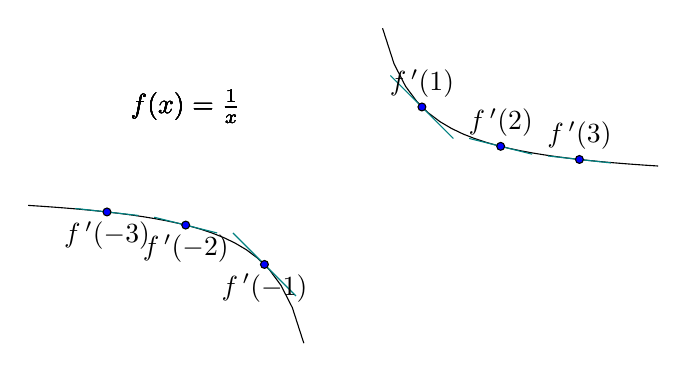
\begin{tikzpicture}
\axes{-4}{4}{-2}{2}
\draw[domain = -4:-0.5] plot (\x, {1/\x});
\draw[domain = 0.5:4] plot (\x, {1/\x});
\foreach \xx in {-3, -2, -1, 1, 2, 3}
{
	\draw[teal, domain = {\xx-0.4}:{\xx+0.4}] plot (\x, {(\xx-\x)/(\xx*\xx) + 1/\xx});
	\ifnum\xx>0
		\filldraw[fill = blue, draw = black] (\xx, {1/\xx}) circle (0.05cm) node[above] {$f\,'(\xx)$};
	\else
		\filldraw[fill = blue, draw = black] (\xx, {1/\xx}) circle (0.05cm) node[below] {$f\,'(\xx)$};
	\fi
	\node at (-2,1) {$f(x) = \frac{1}{x}$};
}
\end{tikzpicture}
\caption{เปรียบเทียบอนุพันธ์ $f\,'(x)$ ของฟังก์ชัน $f(x) = \frac{1}{x}$ เมื่อ $x$ มีค่าลบและบวก}
\label{}
\end{figure}
จากภาพจะเห็นได้ว่า 
\[ f\,'(x) = f\,'(-x) \]
ฉะนั้นฟังก์ชันที่ให้อนุพันธ์เป็น $\frac{1}{x}$ เมื่อ $x$ มีค่าลบคือ $F(x) = \ln (-x)$
\end{frame}

\begin{frame}{สูตรปริพันธ์ของฟังก์ชันเลขชี้กำลัง และฟังก์ชันที่ให้ผลลัพธ์เป็นฟังก์ชันลอการิทึม}
\begin{thm}{สูตรปริพันธ์ของฟังก์ชันเลขชี้กำลัง และฟังก์ชันที่ให้ผลลัพธ์เป็นฟังก์ชันลอการิทึม}{}
\begin{eqnarray*}
\int e^x \, dx &=& e^x + C \\ \pa
%\int a^x \, du &=& (\ln a)a^u + C \\ \pa
\int \frac{1}{x} \, dx &=& \ln |x| + C
\end{eqnarray*}
\end{thm}
\end{frame}

%%%%%%%%%%%%%%
\section[ตรีโกณ]{ปริพันธ์ของฟังก์ชันตรีโกณมิติ}
\frame{\sectionpage}
%%%%%%%%%%%%%%

\begin{frame}[t]{ปริพันธ์ของฟังก์ชันตรีโกณมิติ}
เรามีอนุพันธ์ของฟังก์ชันตรีโกณมิติ
\[ \dx \sin x = \cos x, \qquad \dx \cos x = - \sin x\]
\begin{slide}
ซึ่งแปลงเป็นสูตรปริพันธ์ได้ทันที ดังนี้
\[ \int \cos x \, dx = \sin x + C, \qquad \int - \sin x \, dx = \cos x + C\]
สังเกตว่าในสูตรด้านหลัง เรามีพจน์ $- \sin x$ ซึ่งเราแปลงเป็น $\sin x$ ได้ด้วยการคูณด้วยลบหนึ่งทั้งสมการ จึงได้เป็น
\[\int \sin x \, dx = - \cos x + C\]
\end{slide}
\end{frame}

\begin{frame}{สูตรปริพันธ์ฟังก์ชันตรีโกณมิติ}
\begin{thm}{สูตรปริพันธ์ฟังก์ชันตรีโกณมิติ}{}
\begin{eqnarray*}
\int \sin x \, dx &=& - \cos x + C \\ \pa
\int \cos x \, dx &=& \sin x + C \\ \pa
\end{eqnarray*}
\end{thm}
\end{frame}

\begin{frame}[t]{ปริพันธ์ของฟังก์ชันตรีโกณมิติอื่น}
สำหรับฟังก์ชันอื่น เราไม่สามารถใช้สูตรเดิมได้ทันที เช่น
\[ \dx \tan x = \sec^2 x\]
\begin{slide}
ซึ่งแปลงเป็น 
\[\int \sec^2 x \, dx = \tan x + C\]
ได้ แต่เราไม่สามารถแปลงเป็นสูตรปริพันธ์ของฟังก์ชัน $\tan x$ หรือ $\sec x$ ได้ จึงต้องหาวิธีอื่น นั่นคือถามว่า
\[ \dx F(x) = \tan x \]
\end{slide}
\end{frame}

\begin{frame}[t]
สังเกตว่า 
\[\tan x = \frac{\sin x}{\cos x}\] 
\begin{slide}
ซึงถ้าเราต้องการให้มีพจน์ $\cos x$ เป็นตัวส่วน เราอาจจะใช้สูตร $\dx \ln x = \frac{1}{x}$ และกฏลูกโซ่ได้ ซึงสังเกตว่า
\[ \dx \ln (\cos x) = \frac{1}{\cos x} \left(\dx \cos x\right) = -\frac{\sin x}{\cos x} = - \tan x\]
ซึ่งตรงกับสิ่งที่เราต้องการพอดี จึงสรุปได้ว่า
\[ \int \tan x \, dx = - \ln (\cos x) + C\]
สำหรับฟังก์ชันอื่น ๆ (ได้แก่ $\cot x, \sec x$ และ $\csc x$) จะใช้หลักการเดียวกัน
\end{slide}
\end{frame}

\begin{frame}{สูตรปริพันธ์ฟังก์ชันตรีโกณมิติ}
\begin{thm}{สูตรปริพันธ์ฟังก์ชันตรีโกณมิติ}{}
\begin{eqnarray*}
\int \tan x \, dx &=& - \ln | \cos x| + C = \ln | \sec x| + C\\ \pa 
\int \cot x \, dx &=& \ln | \sin x | + C\\ \pa 
\int \sec x \, dx &=& \ln | \sec x + \tan x | + C \\ \pa 
\int \csc x \, dx &=& \ln | \csc x - \cot x| + C
\end{eqnarray*}
\end{thm}
\end{frame}

\begin{frame}{ฟังก์ชันตรีโกณมิติผกผัน}
สุดท้าย สำหรับฟังก์ชันตรีโกณมิติผกผัน
\[\arcsin, \arccos, \arctan, \arcsec, \arccsc, \arccot\]
เราสามารถหาสูตรได้ แต่เนื่องจากสูตรมีความซับซ้อนและไม่ได้ใช้บ่อยนัก จึงละไว้ในที่นี้ สำหรับสูตรที่มีความสำคัญคือสูตรที่ให้ผลลัพธ์เป็นฟังก์ชันตรีโกณมิติผกผัน เช่น จากอนุพันธ์
\[ \dx \arcsin x = \frac{1}{\sqrt{1-x^2}} \]
แปลงเป็นสูตรปริพันธ์ได้ทันที ดังนี้
\[ \int \frac{1}{\sqrt{1-x^2}} \, dx = \arcsin x + C\]
\end{frame}

\begin{frame}
\begin{thm}{สูตรปริพันธ์ฟังก์ชันตรีโกณมิติที่ให้ผลลัพธ์เป็นฟังก์ชันตรีโกณมิติผกผัน}{}
กำหนดให้ $a$ เป็นค่าคงตัวใด ๆ
\begin{eqnarray*}
\int \frac{1}{\sqrt{a^2-x^2}} \, dx &=& \arcsin\left(\frac{x}{a}\right) + C \\ \pa
&=& \arccos\left(\frac{x}{a}\right) + C \\ \pa
\int \frac{1}{x^2+a^2} \, dx &=& \frac{1}{a}\arctan\left(\frac{x}{a}\right) + C \\ \pa
\end{eqnarray*}
\end{thm}
\end{frame}

\begin{frame}{}
\begin{remark}{หมายเหตุ}
บางครั้งเราจะเห็นสูตรหน้าตาแบบนี้
\[ \int \frac{dx}{\sqrt{1-x^2}} = \arcsin x + C\]
โดยสูตรเหล่านี้มองว่า $dx$ เป็นตัวแปรหนึ่ง ที่สามารถคูณกับตัวเศษได้ นั่นคือ
\[ \frac{dx}{\sqrt{1-x^2}} = \frac{1}{\sqrt{1-x^2}} \, dx\]

ผู้อ่านจะเขียนรูปแบบใดก็ได้ แต่ในเอกสารประกอบการสอนนี้จะเขียน $dx$ ต่อท้ายด้านหลัง เพื่อให้สอดคล้องกับปริพันธ์อื่น
\end{remark}
\end{frame}